\documentclass[
  bibliography=totoc,     % Literatur im Inhaltsverzeichnis
  captions=tableheading,  % Tabellenüberschriften
  titlepage=firstiscover, % Titelseite ist Deckblatt
]{scrartcl}

% Paket float verbessern
\usepackage{scrhack}

% Warnung, falls nochmal kompiliert werden muss
\usepackage[aux]{rerunfilecheck}

% unverzichtbare Mathe-Befehle
\usepackage{amsmath}
% viele Mathe-Symbole
\usepackage{amssymb}
% Erweiterungen für amsmath
\usepackage{mathtools}

% Fonteinstellungen
\usepackage{fontspec}
% Latin Modern Fonts werden automatisch geladen
% Alternativ:
%\setromanfont{Libertinus Serif}
%\setsansfont{Libertinus Sans}
%\setmonofont{Libertinus Mono}
\recalctypearea % Wenn man andere Schriftarten gesetzt hat,
% sollte man das Seiten-Layout neu berechnen lassen

% deutsche Spracheinstellungen
\usepackage{polyglossia}
\setmainlanguage{german}


\usepackage[
  math-style=ISO,    % ┐
  bold-style=ISO,    % │
  sans-style=italic, % │ ISO-Standard folgen
  nabla=upright,     % │
  partial=upright,   % ┘
  warnings-off={           % ┐
    mathtools-colon,       % │ unnötige Warnungen ausschalten
    mathtools-overbracket, % │
},                       % ┘
]{unicode-math}

% traditionelle Fonts für Mathematik
\setmathfont{Latin Modern Math}
% Alternativ:
%\setmathfont{Libertinus Math}

\setmathfont{XITS Math}[range={scr, bfscr}]
\setmathfont{XITS Math}[range={cal, bfcal}, StylisticSet=1]

% Zahlen und Einheiten
\usepackage[
locale=DE,                   % deutsche Einstellungen
separate-uncertainty=true,   % immer Fehler mit \pm
per-mode=symbol-or-fraction, % / in inline math, fraction in display math
]{siunitx}

% chemische Formeln
\usepackage[
version=4,
math-greek=default, % ┐ mit unicode-math zusammenarbeiten
text-greek=default, % ┘
]{mhchem}

% richtige Anführungszeichen
\usepackage[autostyle]{csquotes}

% schöne Brüche im Text
\usepackage{xfrac}

% Standardplatzierung für Floats einstellen
\usepackage{float}
\floatplacement{figure}{htbp}
\floatplacement{table}{htbp}

% Floats innerhalb einer Section halten
\usepackage[
section, % Floats innerhalb der Section halten
below,   % unterhalb der Section aber auf der selben Seite ist ok
]{placeins}

% Seite drehen für breite Tabellen: landscape Umgebung
\usepackage{pdflscape}

% Captions schöner machen.
\usepackage[
  labelfont=bf,        % Tabelle x: Abbildung y: ist jetzt fett
  font=small,          % Schrift etwas kleiner als Dokument
  width=0.9\textwidth, % maximale Breite einer Caption schmaler
]{caption}
% subfigure, subtable, subref
\usepackage{subcaption}

% Grafiken können eingebunden werden
\usepackage{graphicx}
% größere Variation von Dateinamen möglich
\usepackage{grffile}

% schöne Tabellen
\usepackage{booktabs}

% Verbesserungen am Schriftbild
\usepackage{microtype}

% Literaturverzeichnis
\usepackage[style=alphabetic,]{biblatex}
% Quellendatenbank
\addbibresource{lit.bib}
\addbibresource{programme.bib}

% Hyperlinks im Dokument
\usepackage[
  unicode,        % Unicode in PDF-Attributen erlauben
  pdfusetitle,    % Titel, Autoren und Datum als PDF-Attribute
  pdfcreator={},  % ┐ PDF-Attribute säubern
  pdfproducer={}, % ┘
]{hyperref}
% erweiterte Bookmarks im PDF
\usepackage{bookmark}

% Trennung von Wörtern mit Strichen
\usepackage[shortcuts]{extdash}

\title{US3: Doppler-Sonographie}
\author{
  Simon Schulte
  \texorpdfstring{
    \\
    \href{mailto:simon.schulte@udo.edu}{simon.schulte@udo.edu}
  }{}
  \texorpdfstring{\and}{, }
  Tim Sedlaczek
  \texorpdfstring{
    \\
    \href{mailto:tim.sedlaczek@udo.edu}{tim.sedlaczek@udo.edu}
  }{}
}
\publishers{TU Dortmund – Fakultät Physik}

\date{Durchführung: 27.06.2017\\
      Abgabe: 04.07.2017}


\begin{document}

\maketitle
\thispagestyle{empty}
\tableofcontents
\newpage
\setcounter{page}{1}
\section{Zielsetzung}
\label{sec:zielsetzung}
Bei diesem Versuch wird die Schallgeschwindigkeit und Dämpfung von Ultraschall
in Acryl untersucht. Anschließend werden an einem Augenmodell Distanzen gemessen.
\section{Theorie}
\label{sec:theorie}
Als Ultraschall werden Schallwellen mit Frequenzen zwischen $\SI{20}{\kilo\hertz}$
und $\SI{1}{\giga\hertz}$ bezeichnet.
Ihre Intensität nimmt bei der Ausbreitung nach
\begin{equation}
  I \left( x \right) = I_0 \cdot e^{-\alpha x}
  \label{eqn:dämpfung}
\end{equation}
ab. $\alpha$ ist dabei der Absorptionskoeffizient.\\
\\
\noindent
Für die Erzeugung von Ultraschall wird der piezo-elektrische Effekt verwendet.
Hierbei wird ein geeigneter Kristall elekrisch zu Schwingungen angeregt.
Die Resonanz des Kristalls kann dabei auch zur Messung von Ultraschall verwendet
werden.\\
\\
\noindent
Bei Messungen mit Ultraschall gibt es allgemein zwei verschiedene Methoden.
Das Durchschallungs-Verfahren und das Impuls-Echo-Verfahren.\\
Bei dem Durchschallungs-Verfahren werden zwei Ultraschallsonden verwendet.
Die erste agiert als Sender und die zweite als Empfänger. Zischen den
Sonden wird die Probe platziert. Durch Messung der Zeitpunkte der Impulse
lässt sich so bei bekannter Schallgeschwindigkeit die Länge bzw. bei bekannter
Länge die Schallgeschwindigkeit der Probe bestimmen.\\
Bei dem Impuls-Echo-Verfahren wird nur eine Sonde verwendet. Diese agiert
als Sender und Empfänger. Durch Laufzeitmessungen lassen sich auch hier
Länge und Schallgeschwindigkeit der Probe bestimmen. Im Gegensatz zum
Durchschallungs-Verfahren kann hierbei auch die Position von potenziellen
Fehlstellen bestimmt werden.
Da der Schall bei dieser Methode immer den doppelten Weg zurücklegt ergibt sich
für die Strecke
\begin{equation}
  s = \frac{1}{2}\,c\,t
  \label{eqn:strecke}
\end{equation}
\clearpage
\section{Durchführung}
\label{sec:durchführung}
\subsection{Versuchsaufbau}
\label{sec:aufbau}
Der Aufbau besteht aus einem Ultraschallgenerator, an dem zwei Sonden
angeschlossen sind. An einem Drehschalter ist auswählbar, welche Sonden Jeweils
Sender und Empfänger sein sollen. Es stehen mehrere Acrylzylinder und Platten
mit unterschiedlichen Längen bzw. Dicken zur Verfügung. Für das
Durchschallungs-Verfahren liegt ein Keil vor, welcher dafür sorgt, dass
die Zylinder nicht wegrollen. Die Daten der Sonden werden an einem Computer
angezeigt. Daran lassen sich dann die Laufzeiten und Signalamplituden bestimmen.
Für den letzten Versuchsteil wird ein Augenmodell verwendet, wie es in Abbildung
\ref{fig:auge} dargestellt ist.
\begin{figure}[H]
  \centering
  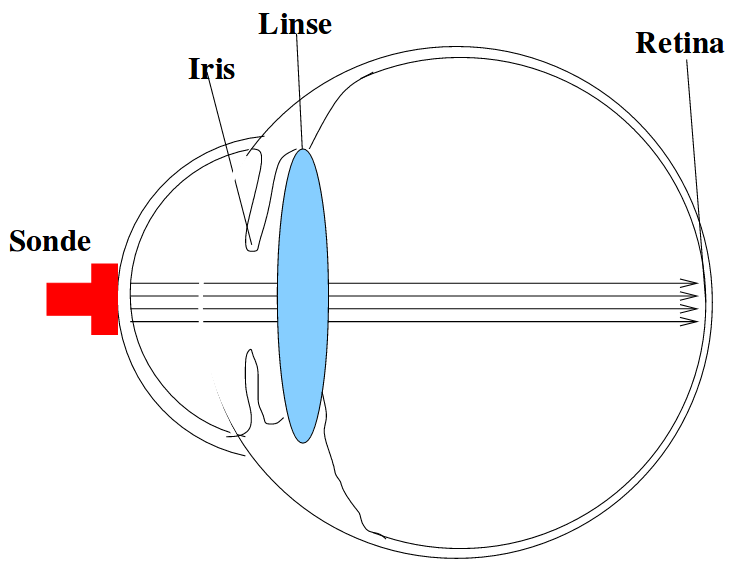
\includegraphics[width=0.5\textwidth]{Augenmodell.png}
  \caption{Schematische Darstellung des Augenmodells. \cite{anleitung}}
  \label{fig:auge}
\end{figure}
\noindent
Für die Zylinder und Platten wurden vorab folgende Längen gemessen:
\begin{table}
  \centering
  \caption{Zylinderlängen.}
  \label{tab:größen}
  \sisetup{table-format=2.3}
  \begin{tabular}{S[table-format=1.0] S}
    \toprule
    {Zylinder/Platte Nr.} & {Länge/Dicke in \si{\centi\meter}} \\
    \midrule
    1 &  3.115 \\
    2 &  4.045 \\
    3 &  6.160 \\
    4 &  7.086 \\
    5 &  8.045 \\
    6 & 10.240 \\
    7 & 12.055 \\
    a &  0.610 \\
    b &  1.195 \\
    \bottomrule
  \end{tabular}
\end{table}\\
\noindent
Zylinder Nr.4 wird dabei aus einem Zylinder der Länge $\SI{3}{\centi\meter}$
und einem der Länge $\SI{4}{\centi\meter}$ zusammengesetzt und die Buchstaben
stehen für die Acrylplatten.
\clearpage
\subsection{Versuchsablauf}
\label{sec:ablauf}
Zuerst wird mit dem Impuls-Echo-Verfahren die Laufzeit und die Amplitude der
Impulse in den verschiedenen Zylindern gemessen. Damit lässt sich die
Schallgeschwindigkeit in Acryl und der entsprechende Absorptionskoeffizient
bestimmen.
Anschließend werden alle Zylinder außer Nr.4 mit dem Durchschallungs-Verfahren
erneut vermessen. Hierbei wird nur die Laufzeit notiert.\\
\\
\noindent
Nun werden die beiden Acrylplatten aufeinander und Zylinder Nr.2 auf den beiden
Platten platziert. Von oben wird dann per Impuls-Echo-Verfahren ein Cepstrum
aufgenommen. Dieses zeigt ein Spektrum aus Laufzeiten, die durch mehrfache
Reflexion entstehen. Anhand dieser kann die Dicke der Platten bestimmt werden.\\
\\
\noindent
Zuletzt werden an einem Augenmodell per Impuls-Echo-Verfahren die Abstände
zwischen Iris, Linse und Retina bestimmt.
\clearpage
%Auswertung
\end{document}
